\subsection{Accommodation}
\label{sec:related_work:accommodation}

Previous AR displays that propose technologies to provide accommodation are broadly classified and their limitations are mentioned: (1) \emph{Varifocal Displays:}~\cite{Dunn2017Wide,Aksit2017Near} Provides synthetic focus cues, requires to track accommodation-state of the eye, and has latency in moving the in-focus plane. (2) \emph{Multifocal Displays:}~\cite{Akeley2004,Narain2015optimal} Few focal planes which leads to partly synthetic focal cues and reduced spatial resolution for content in-between the few focal planes. (3) \emph{Light-field Displays:}~\cite{Maimone2014} Poor spatial resolution and narrow depth-range. (4) \emph{Holographic Displays:}~\cite{Maimone2017Holographic} Very small eyebox, narrow depth-range.

%\input{media/fig_volumetric_results.tex}
\begin{comment}
 \begin{itemize}
 \item \emph{Varifocal Displays:}~\cite{Dunn2017Wide,Aksit2017Near} Provides synthetic focus cues, requires to track accommodation-state of the eye, and has latency in moving the in-focus plane.
 \item \emph{Multifocal Displays:}~\cite{Akeley2004,Narain2015optimal} Few focal planes which leads to partly synthetic focal cues and reduced spatial resolution for content in-between the few focal planes.
 \item \emph{Light-field Displays:}~\cite{Maimone2014} Poor spatial resolution, frame-rates, and narrow depth-range,
 \item \emph{Holographic Displays:}~\cite{Maimone2017Holographic} Very small eyebox, narrow depth-range.
 \end{itemize}
\end{comment}

\emph{Volumetric AR display}, developed and demonstrated as part of this dissertation, is a multifocal display with 280 single-color binary image planes -- a significant improvement upon previous multifocal displays. The volumetric AR display can present full-color imagery (24 bit-depth) spanning a large volume (15 cm to 400 cm with 45$^\circ$ Field-of-View) composed of 280 binary images, each of which has the native resolution of the display (1024 $\times$ 768), and does not require eye-tracking.

\subsection{Occlusion}
\label{sec:related_work:occlusion}

\emph{Light-field occlusion display}~\cite{Maimone2013} attempts to provide depth-dependent occlusion by presenting a 4D light field occlusion mask using stacked LCD layers placed out of focus in front of the eye, where the occluding patterns are calculated by light field factorization algorithms~\cite{Lanman2010, Wetzstein2012}. While theoretically capable of presenting depth-dependent occlusion cues, this approach's use of LCD panels causes severe diffraction and deterioration of the real-world's view. \emph{Fixed-focus occlusion displays}~\cite{Kiyokawa2003} can preserve a high-quality of the see-through view, but present the occlusion mask at a fixed distance.
\begin{figure}
\centering
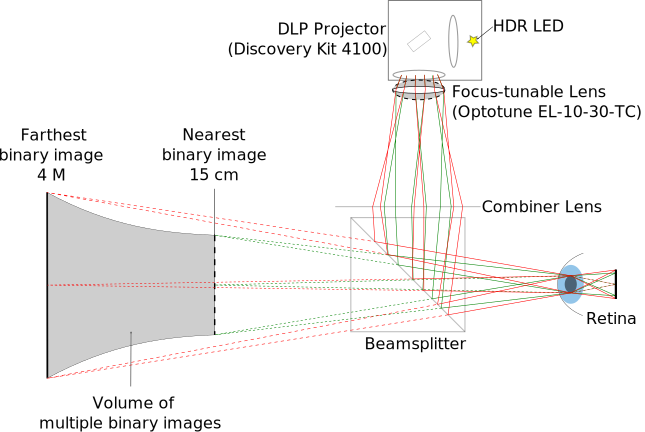
\includegraphics[width=0.99\columnwidth]{images/volumetric/proposedCandidate}
%\fbox{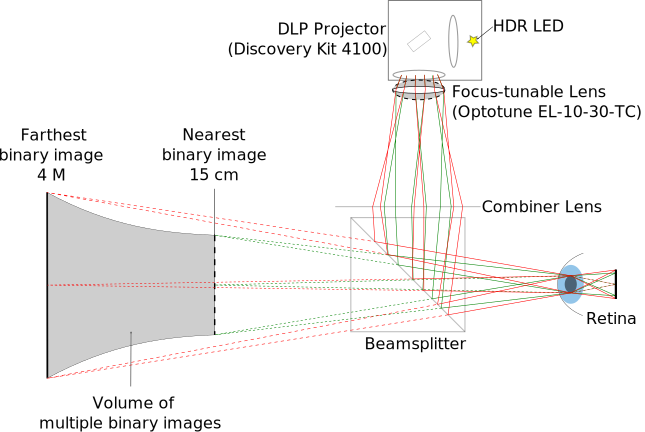
\includegraphics[width=0.46\textwidth]{images/volumetric/proposedCandidate}}
\caption[Volumetric NED: optics overview]{Figure shows an overview of the hardware and operation of our NED. The NED is composed of a high-speed HDR LED, high-speed projector, focus-tunable lens, and other common optical components. The NED's optics, rendering pipeline, and the synchronized operation of its active components (HDR LEDs, DMD, focus-tunable lens) work together to present a color volume spanning 15cm (6.7 diopters) to 4M (0.25 diopters).}
\label{fig:volumetric:proposedCandidate}
\end{figure} 

\emph{Varifocal occlusion display}, developed and demonstrated as part of this dissertation, is an extension of \emph{fixed-focus occlusion displays}, where the single occlusion image plane is now moveable in depth.



\begin{comment}
\section{Literature on the importance of depth cues for AR displays}

\cite{sielhorst2008advanced} provide a good set of references on depth perception studies. \cite{sielhorst2008advanced} also provide a good summary of \cite{cutting1995perceiving} which in turn is a seminal paper about the different types of depth cues and their relative importance. The summary: Occlusion is the most important depth cue even though it is only an  because because it can only reveal the order but not a relative or absolute distance. \cite{sielhorst2008advanced} call it ``interposition''. \cite{sielhorst2008advanced}.
\end{comment}

\begin{itemize}
\item \emph{Varifocal Displays:}~\cite{Dunn2017Wide,Aksit2017Near} Provides synthetic focus cues, requires to track accommodation-state of the eye, and has latency in moving the in-focus plane.
\item \emph{Multifocal Displays:}~\cite{Akeley2004,Narain2015optimal} Few focal planes which leads to partly synthetic focal cues and reduced spatial resolution for content in-between the few focal planes.
\item \emph{Light-field Displays:}~\cite{Maimone2014} Poor spatial resolution, frame-rates, and narrow depth-range,
\item \emph{Holographic Displays:}~\cite{Maimone2017Holographic} Very small eyebox, narrow depth-range.
\end{itemize}
